\documentclass[UTF8]{ctexart}

\usepackage{amsmath}
\usepackage{subfigure}
\usepackage{hyperref}

\usepackage[graphicx]{realboxes}


\title{Image Caption 学习笔记 Week 1}
\author{高崧淇}
\date{\today}

\begin{document}

\maketitle
\tableofcontents

\section{Image Caption 简介}

Image Caption,就是给模型输入一张图片,模型输出一段描述性文字。类似于小学语文的“看图说话”任务。
对于人类来说,图像描述是简单而自然的一件事,但对于机器来说这项任务却充满了挑战性。
因为机器不仅要能检测出图像中的物体,而且要理解物体之间的相互关系(此处具有很强的二义性,因为
根据描述者的关注点和思考角度不同,现实中的图片存在多种描述方式),最后还要用合理的自然语言表达出来。

\section{Show and Tell}
Image Caption属于图片分类和文本生成的交叉任务,Show and Tell: A Neural Image Caption Generator~\cite{show} 把当时
CV领域和机器翻译领域的进展结合起来,提出来用于Image Caption任务的模型。

该模型是端到端的设计,整体采用encoder-decoder架构。图像表示使用ILSVRC 2014分类比赛的冠军模型~\cite{bn}编码,文本生成
部分使用LSTM解码。

\subsection{Model}

作者提出了直接最大化给定图像输出正确描述的概率,如 Eq.~\ref{eq:eq1}

\begin{equation}
    \theta^* = arg \mathop{max}\limits_{\theta} \sum_{(I,S)} log\;p(S|I;\theta )\label{eq:eq1}
\end{equation}

此处$\theta$是模型的参数,$I$ 是图像,$S$ 是正确描述句子。因为句子长度不定,所以上式可
根据链式法则展开为 Eq.~\ref{eq:eq2}

\begin{equation}
    log\;p(S|I) = \sum_{t=0}^{N} log\;p(S_t|I,S_0,...,S_{t-1}) \label{eq:eq2}
\end{equation}

而RNN网络可以用于 Eq.~\ref{eq:eq3}这种当前输出依赖于前序输出的结构,不过考虑到梯度爆炸的问题,
作者选用了LSTM。

\begin{equation}
    h_{t+1}=f(h_t,x_t) \label{eq:eq3}
\end{equation}

模型架构如图~\ref{fig:1}。


\begin{figure}
    \centering
    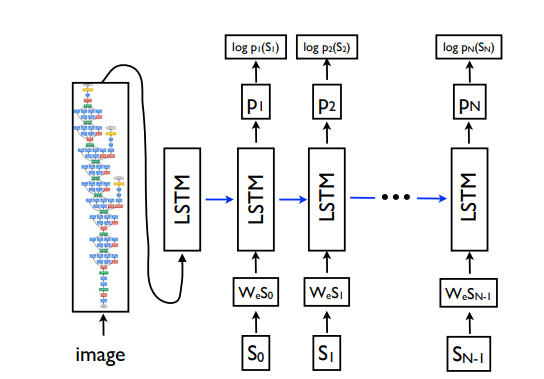
\includegraphics[width=\textwidth]{dddd}
    \caption{Architecture of the model.}
    \label{fig:1}
\end{figure}

\subsection{Training}

文章中使用One-hot向量$S_t$表示每个单词, 用特殊记号$S_0$和$S_N$表示句子的开始和终止,
图片与词语分别使用CNN和词嵌入映射到同一个空间。经过实验验证,图片只在$t = -1$的时
候输入进网络一次的效果比每个时间都喂进图片效果好。网络的Loss函数如下

\begin{equation}
    L(I,S)=-\sum_{t=1}^N log\;p_t(S_t)
\end{equation}

\subsection{Inference}
推理方法有两种,直接采样(只取第一个)和集束搜索。

集束搜索~\cite{beam}:在当前级别的状态下计算所有可能性,并按照递增顺序对他们进行排序,
但只保留一定数量的可能结果(依据Beam Width决定数量),接着根据这些可能结果进行扩展,
迭代以上的动作直到搜索结束并返回最佳解(具有最高概率的那个)。可以理解搜索树的剪枝。

\subsection{Experiments}
作者使用了BLEU-4 METEOR CIDER和人类评价的方式,Pascal VOC 2008、Flickr8k、Flickr30k、
MSCOCO、SBU几个数据集上做了测试,获得了如图~\ref{fig:2}的性能。


\begin{figure}
    \centering
    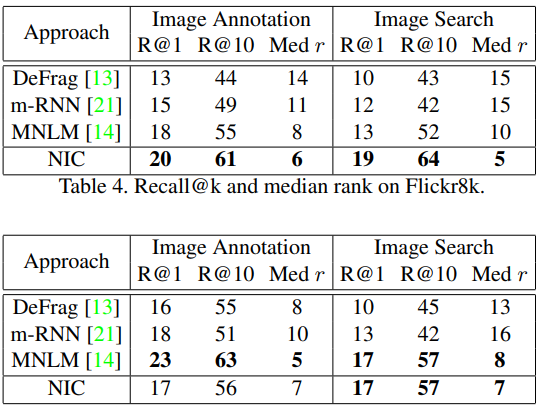
\includegraphics[width=2.5in]{111}
    \caption{性能表现}
    \label{fig:2}
\end{figure}

\section{Knowing When to Look}
Knowing when to look: Adaptive attention via a visual sentinel for image captioning~\cite{when}
这篇文章是在注意力应用于编解码器架构后提出的一种改进。主要思路是把注意力机制应用在了
时间步上,让模型判断当前时间步下应该更侧重于图像特征还是前序文本。
改进了LSTM单元,如图~\ref{fig:3},这种改进借鉴Resnet的残差连接思想。


\begin{figure}
    \centering
    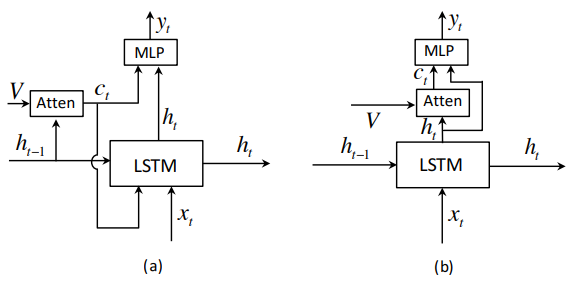
\includegraphics[width=2.5in]{attn_lstm.png}
    \caption{改进的注意力LSTM单元}
    \label{fig:3}
\end{figure}


\section{总结}
经过本周的学习,主要总结几点启发如下:
\begin{itemize}
    \item 采用机器翻译的思路,图像描述可以看做把图片翻译为文本
    \item 采用预训练的图片特征层
    \item 编解码器结构可以很好的适应这种“翻译”任务
    \item 对比人工评价的得分,发现BLEU指标并不能很好的表征描述文本的好坏
\end{itemize}


\begin{thebibliography}{8}
    \bibitem{show}
    Vinyals, Oriol, et al. "Show and tell: A neural image caption generator." Proceedings of the IEEE conference on computer vision and pattern recognition. 2015.

    \bibitem{bn}
    Ioffe, Sergey, and Christian Szegedy. "Batch normalization: Accelerating deep network training by reducing internal covariate shift." International conference on machine learning. PMLR, 2015.

    \bibitem{beam}
    BeamSearch
    \url{https://zhuanlan.zhihu.com/p/58526617}

    \bibitem{when}
    Lu, Jiasen, et al. "Knowing when to look: Adaptive attention via a visual sentinel for image captioning." Proceedings of the IEEE conference on computer vision and pattern recognition. 2017.


\end{thebibliography}

\end{document}
